\documentclass[twoside,12pt]{article}

\usepackage[nottoc,numbib]{tocbibind}

\usepackage{amsmath,amsfonts,amsthm,fullpage}
\usepackage{amsmath}
\usepackage{amssymb}
\usepackage{listings}
\setlength{\parindent}{0pt}
\usepackage{graphicx}
\usepackage{bm}
\usepackage[section]{placeins}
\usepackage{multirow}% http://ctan.org/pkg/multirow
\usepackage{hhline}% http://ctan.org/pkg/hhline

% Use the standard article template.
%
% The geometry package allows for easy page formatting.
\usepackage{geometry}
\geometry{letterpaper}
% Load up special logo commands.
\usepackage{doc}
% Package for formatting URLs.
\usepackage{url}
% Packages and definitions for graphics files.
\usepackage{epstopdf}
\DeclareGraphicsRule{.tif}{png}{.png}{`convert #1 `dirname #1`/`basename #1 .tif`.png}

\def\argmin{\operatornamewithlimits{arg\, min}}
\newcommand{\rbr}[1]{\left(#1\right)}
\newcommand{\cbr}[1]{\left\{#1\right\}}
\newcommand{\Ncal}{\mathcal{N}}
\renewcommand{\familydefault}{\sfdefault}
\newcommand{\setof}[1]{\ensuremath{\left \{ #1 \right \}}}
\newcommand{\tuple}[1]{\ensuremath{\left \langle #1 \right \rangle }}

%
% Set the title, author, and date.
%
\title{
2016\\
Kaggle Competition - Predict the relevance of search results on homedepot.com 
}
\author{Ajay D'Souza (adsouza31)}
\author{
  D'Souza, Ajay\\
  \texttt{ajaydsouza@gatech.edu}
}
\date{\today}


\iffalse
*------------------------------------------------------------*
  These are the instructions for the Report
*------------------------------------------------------------*

The final written report shall not be longer than 30 pages, and the body of the report (without
appendix and figures/tables) is generally 5 to 15 pages. Only very relevant plots and tables shall be included
in the body of the report, and the rest should go to Appendix. When writing up your summary report, it is
useful to ask yourself the following questions: What is the work? Why is it important? What background
is needed? How will the work be presented?
Here is a suggested format for your summary report.
1. Title Page: Project Title, author(s) (your name, the last five digits of your student ID, and email
address), the submission date, course name/number;
2. Abstract: informative summary of the whole report (100-300 words).
3. Introduction includes problem description and motivation, data mining challenge(s), problem solving
strategies, accomplished learning from the applications and outline of the report.
4. Problem Statement or Data Sources: cite the data sources, and provide a simple presentation of
data to help readers understand the problem or challenge(s).
5. Proposed Methodology: explain (and justify) your proposed data mining strategies.
6. Analysis and Results: present key findings when executing the proposed data mining methods. For
the benefit of readability, detailed results should be placed in the Appendix. Reference of computer
softwares to implement your proposed data mining methods (even it is a web page) should be given.
7. Conclusions: Draw conclusions from your data mining practice. Unfinished or possible future work
could be included (with proper explanation or justification).
At the end of conclusion section, please add a subsection for lessons you learned from
this project (or this course).
8. Appendix: This section only includes needed documents to support the presentation in the report.
Feel free to divide it into several subsections if necessary. Do NOT dump all computer outputs unorganized
here.
9. Bibliography and Credits.
Parts 3-6 constitute the meat of the paper for your primary audience. Usually, as with fictional boss in
this example, your audience is intelligent but unschooled in Data Mining or Statistics. So these parts should
have as little technical material as you can possibly get away with.
It is appropriate, and even recommended, to refer the reader to the appendix in part 8 if you need to
provide a more technical explanation for something. Part 8 is your secondary audience - me - and should
follow closely enough the ”story” of parts 4 􀀀 6 that it is easy for me to see what technical material backs
up with results and discussion.
It is not necessary to number these parts 1-9 or name them as-above-mentioned. Please feel free to merge
some parts or provide more informative section names if it seems natural to do so.
A good on-line resource for writing reports is http://www.ccp.rpi.edu/. This site has links to writing
centers at universities around the country, many of which in turn have pages that describe how to put
together different types of reports.


\fi

\begin{document}

\maketitle

% Add an abstract.
\begin{abstract}
The goal of this Kaggle Competition is to develop an algorithm that matches the results of the manual rating score for determining the relevance of a search string to a given product
\end{abstract}

% Add various lists on new pages.
\pagebreak
\tableofcontents

\pagebreak
\listoffigures
\listoftables

% Start the paper on a new page.
\pagebreak



%
% Body text.
%
\section{Introduction}
\label{Introduction}
\begin{itemize}
\item
\url{www.kaggle.com} has a an open competition for \textbf{\textit{Home Depot Product Search Relevance }} at \url{https://www.kaggle.com/c/home-depot-product-search-relevance}. At Home Depot humans rate the relevancy of a search string to a product by assigning an rating score to a tuple of \tuple{product,searchstring}. The on-line search algorithm at Home Depot is evaluated and tuned to use this manual rating score. Manual rating however is a slow process and will not scale. Through this competition Home Depot is seeking to find an algorithm than can learn from the manual rating process and mimic it.
\item
Home depot has provided a training data set that has a tuple of \tuple{product,searchstring} along with a rating score for each tuple. The rating score is in the range of $1\dots3$, with 1 indicating that the product is irrelevant to the search string and 3 indicating that the search string is fully relevant to the product. We need to train a model to be able to predict this  rating score for a tuple of \tuple{product,searchstring}. 
\item
A test data set comprising of tuples of \tuple{product,searchstring} is provided. The model needs to make predictions for this test set. The test results set are to be submitted and will be evaluated using RMSE (Root Mean Square Error). 
\item
It should be noted that the goal is not to search for the best product for a search string, but instead to develop a model which predicts a rating score that matches the manual rating score for a tuple of \tuple{product,searchstring}.
\end{itemize}

  
\section{Problem Definition}
\label{Problem Definition}
\subsection{Source of Data}
\label{source_of_data}
\begin{itemize}
\item
The data for the competition is provided on Kaggle at \url{https://www.kaggle.com/c/home-depot-product-search-relevance/data}. The data comprises of training data, test data, a catalog of product descriptions, product attributes, instructions for manual rating.  The table $\eqref{p_tab_1}$ lists the data files provided along with a description as mentioned on \url{https://www.kaggle.com}

\begin{table}[h]
\centering
\resizebox{\textwidth}{!}{
	\begin{tabular}{|r|l|}
	\hline
	train.csv & The training set, contains products, searches, and relevance scores \\
	\hline
	test.csv & The test set, contains products and searches. You must predict the relevance for these pairs\\
	\hline
	product\_descriptions.csv & Contains a text description of each product. You may join this table to the training or test set via the product\_uid\\
	\hline
	attributes.csv & Provides extended information about a subset of the products (typically representing detailed technical specifications). Not every product will have attributes.\\
	\hline
	sample\_submission.csv & A file showing the correct submission format \\
	\hline
	relevance\_instructions.docx & The instructions provided to human raters\\
	\hline
	\end{tabular}
	}
	\caption[]{Data for - \textbf{Home Depot Product Search Relevance} Competition}
	\label{p_tab_1}
\end{table}


\item
Table $\eqref{p_tab_2}$ provides a detailed description of the contents of the data provided in the training dataset, product description and product attributes files.
\FloatBarrier
\begin{table}[h]
\centering
\resizebox{\textwidth}{!}{
	\begin{tabular}{|r|l|}
	\hline
	id & A unique Id field which represents a (search\_term, product\_uid) pair\\
	\hline
	product\_uid & An id for the products\\
	\hline
	product\_title & The product title\\
	\hline
	product\_description & The text description of the product (may contain HTML content)\\
	\hline
	search\_term & The search query\\
	\hline
	relevance & The average of the relevance ratings for a given id\\
	\hline
	name & An attribute name\\
	\hline
	value & The attribute's value\\
	\hline
	\end{tabular}
	}
	\caption[]{Data description - \textbf{Home Depot Product Search Relevance} Competition}
	\label{p_tab_2}
\end{table}
\end{itemize}



\section{Data Cleanup}
\label{cleanup}
The following data clean up was performed
\begin{enumerate}
	\item
	There are 13 distinct values for the response variable $relevance$ in the training set. Figure $\eqref{r_c_b}$ is a bar plot of the count for each of the $13$ values of the response variable in the training data set. As can be seen over $99.9\%$ of the values are taken by seven values of the response variable. The remaining six account for less than $.01\%$ of the rows in the training data. This data was considered as out-lier data and rows for this data where cleaned up from the training data set. The retained seven values are also well rounded numbers. This indicates that most of the rating scores might have been actually be the scores of a single rater rather than a average of multiple raters.
	\FloatBarrier
	\begin{figure}[!htbp]
		\centering
		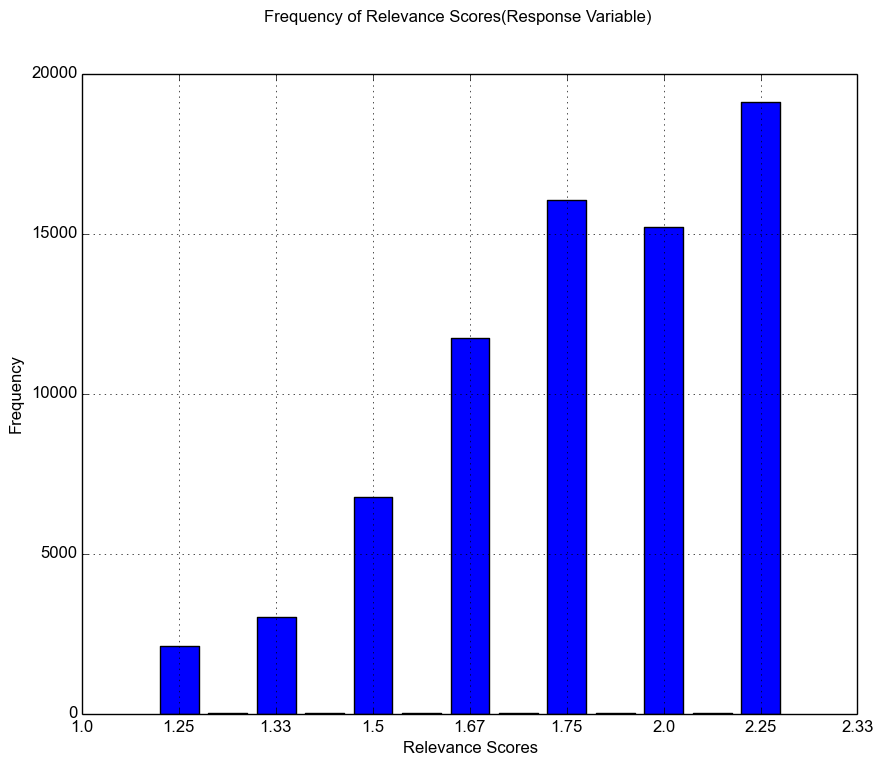
\includegraphics[scale=.43]{DataVisualization/relv_plot.png} 
		\caption{Frequency of Relevance Score Values (Response) }
		\label{r_c_b}
	\end{figure}
	\item
	The text and training data provided is in English. All figures, numeric data, escape sequences, Unicode characters and any other special characters where converted to text or replaced by empty space from the test and training data.   
	\item
	Text data is further cleaned to remove stop words, words less than 2 characters. All text data is then converted to the same lower case.
	\item
	All text in  the test and training dataset for the fields search string, product title, product description and product attributes is stemmed. Porter stemmer implementation in python is used for stemming.
\end{enumerate}



\section{Exploratory Data Analysis and Generating the Feature Vector}
\label{exploratory}
Once we have the cleaned and stemmed data we need to represent each row into a feature vector of numeric or categorical data. We can use this feature vector representation for fitting a learning model.  An exploration of the text strings in attributes shows that the string $\textit{mfg brand name}$ is the most common n-gram for a bullet point in attributes. Its attribute value is taken to be the brand and is extracted and added as a column for each record.
	
For the predictors we have 4 bodies of cleaned stemmed text data for each record.
\begin{enumerate}
		\item 
		The Product Title
		\item
		The Product Description
		\item
		The Product Attributes
		\item
		Brand
		\item
		The Search String
\end{enumerate}

\subsection{Generation of Feature Vectors}
\label{feature_vectors}
The following exploratory data plots will help to engineer some of the features. The plots plot the various possible metrics for the data versus the relevance values. Since we have 13 distinct relevance values in the training data, each point in the plot will represent an average of that metric across all records that have that relevance value. Records will be grouped by their by their relevance score and their metric value will be averaged for that group to get a single value of that metric for a given relevance score to be used for these plots.

\begin{itemize}
	
\FloatBarrier
\item 
Figure $\eqref{wc_v_r}$ is a word count plot. It plots the word count in each of the fields of product title, product description and search string averaged for each of the 13 values of the response variable. The word count does not appear to show much of an explicit correlation to the relevance score except for product description for which there is a slight increase in relevance scores as the words in product description increases.
		
		\begin{figure}[!htbp]
			\centering
			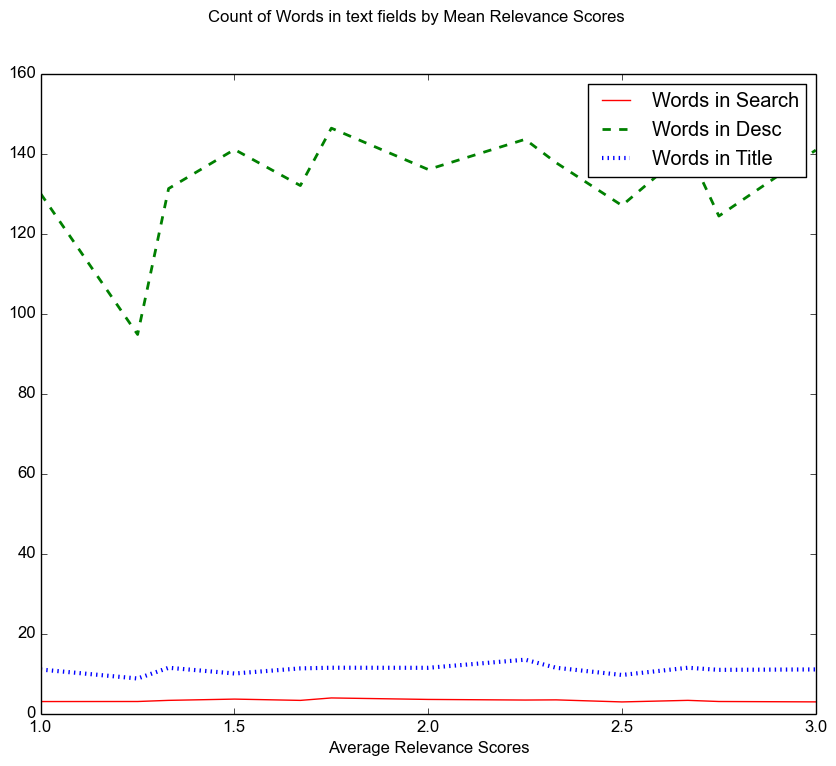
\includegraphics[scale=.43]{DataVisualization/length_relv_plot.png} 
			\caption{Count of words in different text fields Vs Mean Relevance Score}
			\label{wc_v_r}
		\end{figure}

		
\FloatBarrier
\item 
Figure $\eqref{wc_s_m_r}$ plots the average count of matching n-grams between the search string in a record with each of the fields of product title, product description, product brand in that record. Again the average is taken across the records for each of the 13 values of the response variable. As can be seen in the plot, a slight increase in relevance scores as the count of matching n-grams between search and title, description and brand increases.
\FloatBarrier
\begin{figure}[!htbp]
	\centering
	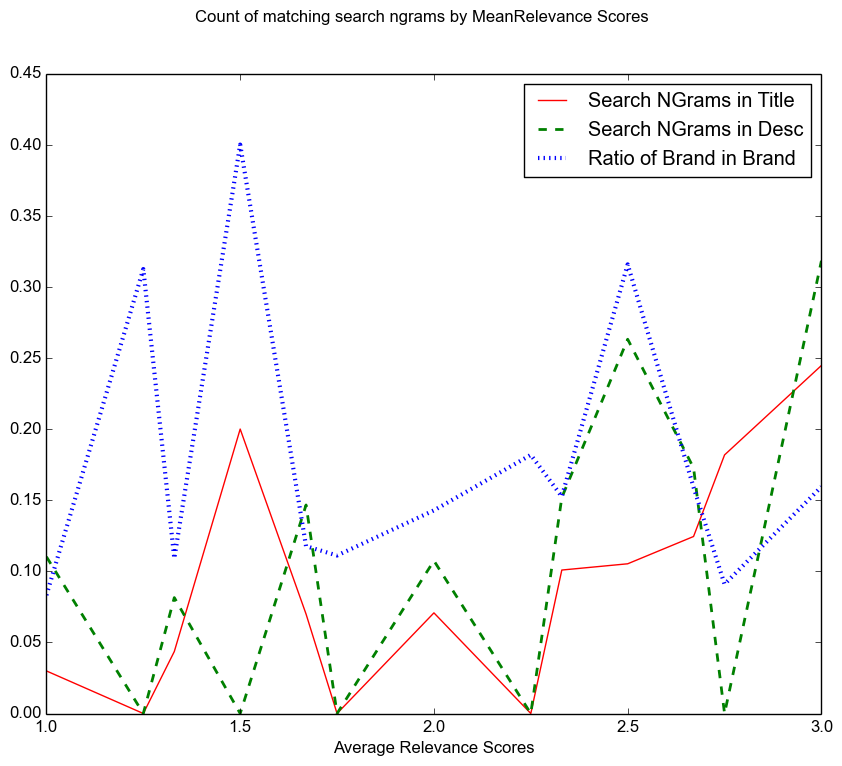
\includegraphics[scale=.43]{DataVisualization/ngrams_relv_plot.png} 
	\caption{Count of matching n-grams between search and text fields by Relevance Values}
	\label{wc_s_m_r}
\end{figure}

\FloatBarrier
\item 
Figure $\eqref{r_s_m_r}$ is a more normalized representation of the matching word count between search and the text in title, description and brand. The ratio of the count of matching words to the total number of words in the search string is plotted. The values grouped by relevance and are averaged for each of the 13 distinct relevance values. There is a pronounced increase in relevance score as the ratio of the word match increases for the title and description fields.
\FloatBarrier
\begin{figure}[!htbp]
	\centering
	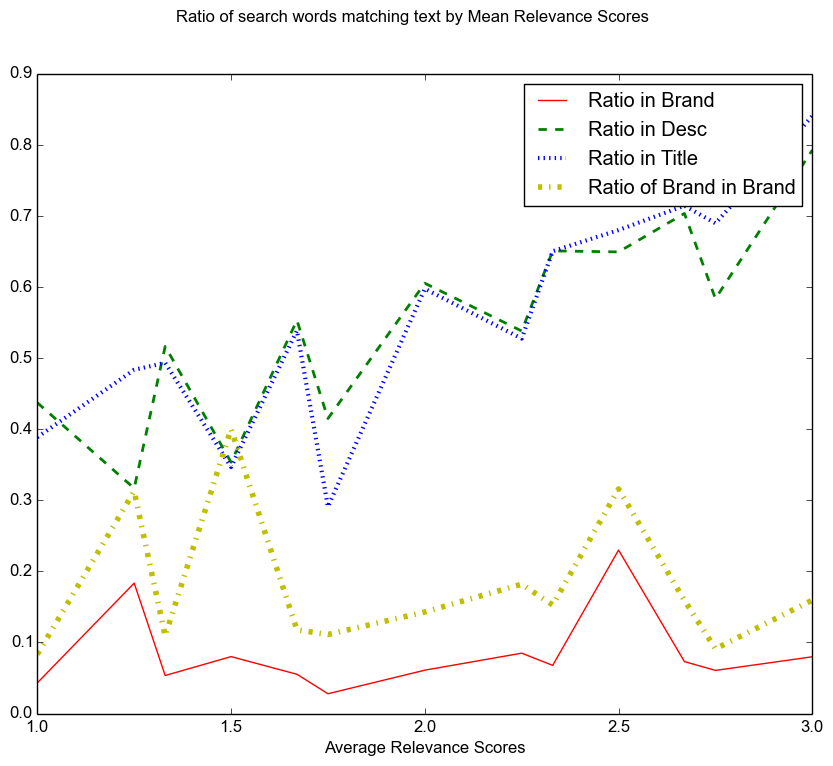
\includegraphics[scale=.43]{DataVisualization/ratio_relv_plot.png} 
	\caption{Ratio of word count matching with search to the total words in search by Relevance}
	\label{r_s_m_r}
\end{figure}

\FloatBarrier
\item 
Figure $\eqref{j_s_m_r}$ plots the Jaccard Coefficient between the words in search string to each of the text fields of product title, product description and brand. The values are grouped and averaged by relevance score values. The Jaccard coefficient for the product title has a strong positive correlation to the relevance score. The Jaccard coefficient for brand and description with search appears to fairly neutral to slightly positive in its correlation to the relevance score values.
\FloatBarrier
\begin{figure}[!htbp]
	\centering
	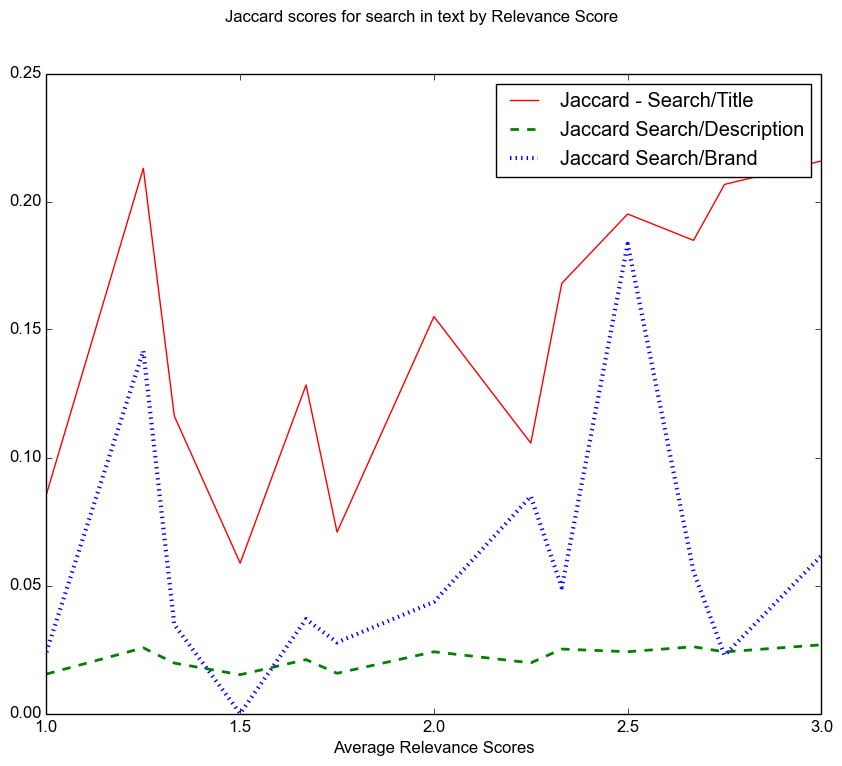
\includegraphics[scale=.43]{DataVisualization/jaccrd_relv_plot.png} 
	\caption{Jaccard Coefficient between search and text fields by Relevance}
	\label{j_s_m_r}
\end{figure}

\FloatBarrier
\item 
Figure $\eqref{sp_pid_r}$ scatter plots count of a product id versus the average relevance score for that product id. Product ids are first grouped and counted and then the mean of their relevance is taken for this plot. The plot shows that as the product is seen in more records in the training data, its average relevance value across the records also increases. Product ids with a low count have a much wider spread of their relevance values, while those with a higher count have a narrower band of relevance values.
\FloatBarrier
\begin{figure}[!htbp]
	\centering
	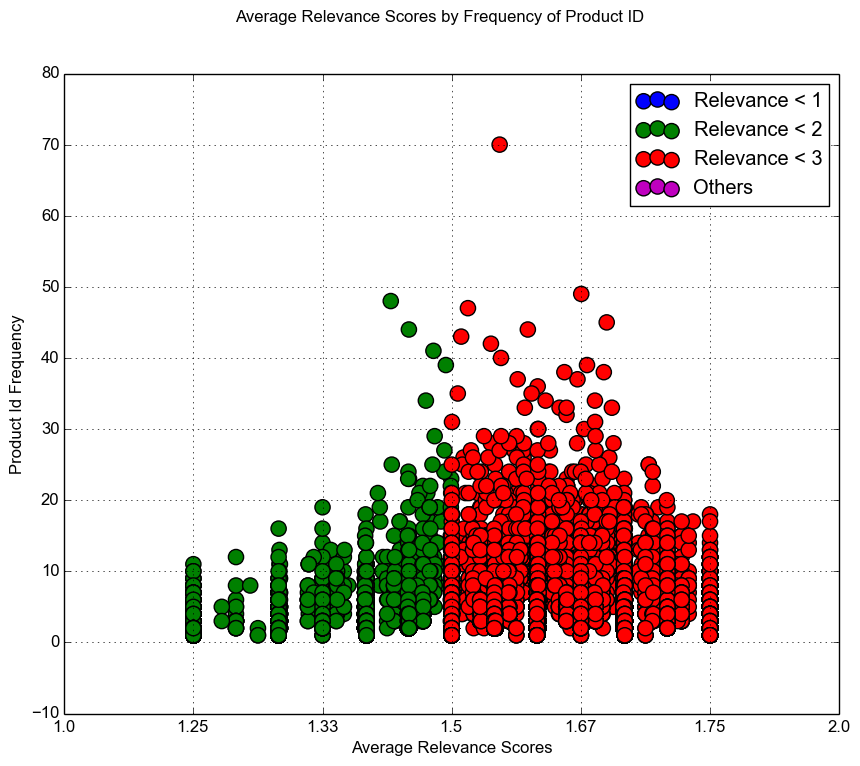
\includegraphics[scale=.43]{DataVisualization/pid_relv_cnt_plot.png} 
	\caption{Scatter Plot of the count of product id Vs Mean Relevance}
	\label{sp_pid_r}
\end{figure}

\FloatBarrier
\item 
Figure $\eqref{lw_s_r}$ is a plot of the word count of the words in title and description matching the last word in search. As discussed earlier the records are grouped by their relevance values and an average of this metric value is taken across the records with the same relevance for this plot. There is a very strong and positive correlation between the count of matching last search words to the relevance score as can be seen in this plot.
\FloatBarrier
\begin{figure}[!htbp]
	\centering
	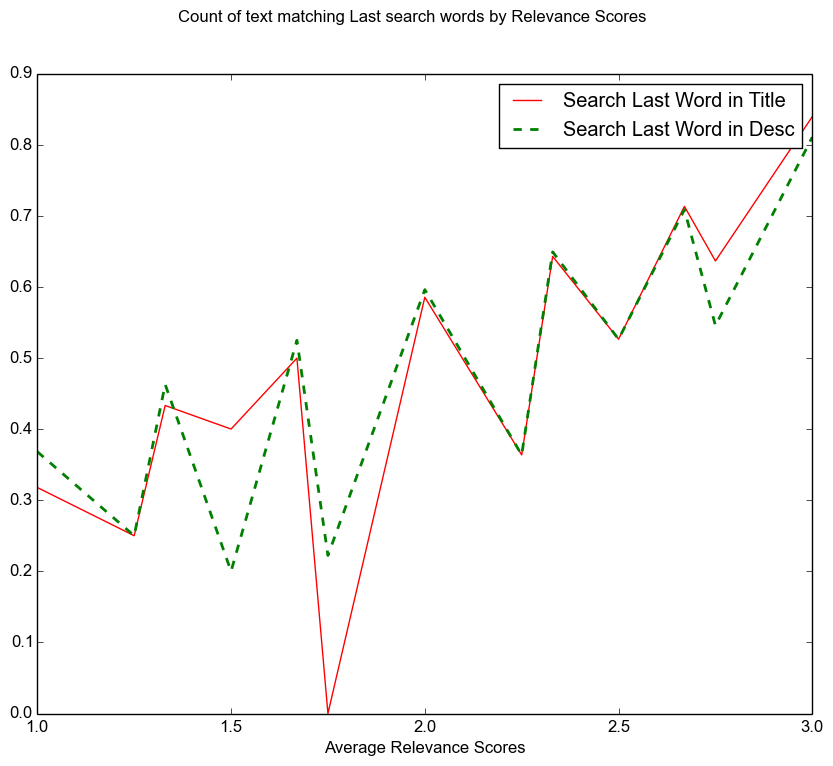
\includegraphics[scale=.43]{DataVisualization/lastw_relv_plot.png} 
	\caption{Count of matching words in text fields to last the word in search Vs Relevance}
	\label{lw_s_r}
\end{figure}

\FloatBarrier
\item 
Figure $\eqref{sg_s_r}$ is a plot of the count of all the matching segments between text in search to the text in title. The count is grouped and averaged by relevance values. The correlation is neutral with a slight increase for the mid range of relevance scores. It does not appear to be a simple linear correlation.
\FloatBarrier
\begin{figure}[!htbp]
	\centering
	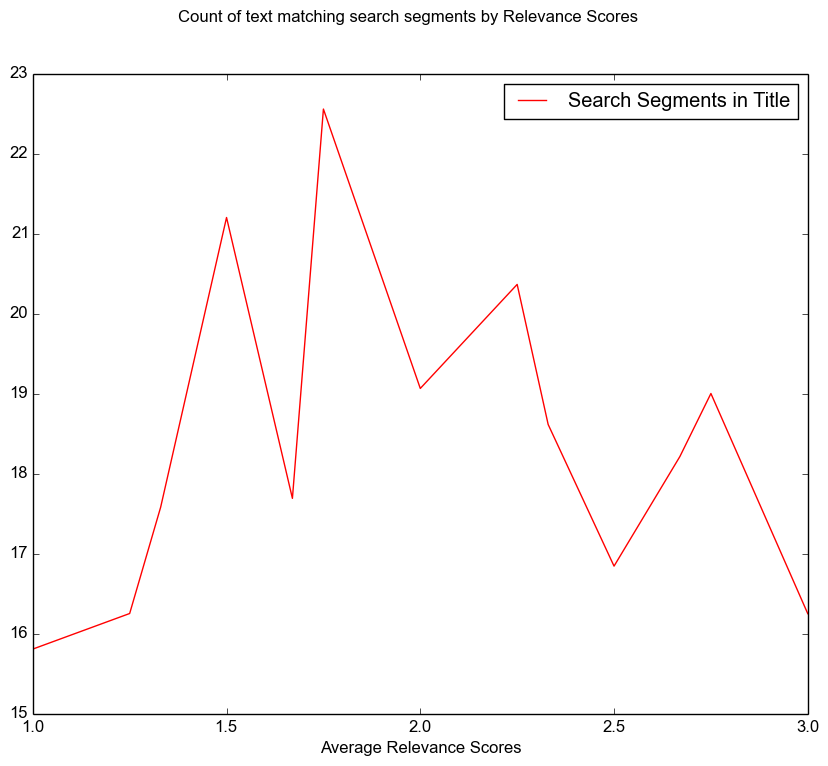
\includegraphics[scale=.43]{DataVisualization/srch_seg_relv_plot.png} 
	\caption{Count of matching segments between search and product title by Relevance}
	\label{sg_s_r}
\end{figure}

\FloatBarrier
\item
From the rating guidelines document a search word matching brand is mentioned as an important criterion for a high rating score. As discussed earlier, brand is extracted from the $\textit{mfg brand name}$ attribute value as a text string. From these brand names we build a list of unique brand names and identify each unique brand name by a numeric brand id. We engineer a feature for the brand by populating back the brand id for the brand name string in the record. 

\item
Thus based on the discussion so far the following 22 features will be engineered for each record.
\begin{table}[h]
	\centering
	\resizebox{\textwidth}{!}{
		\begin{tabular}{|r|l|}
			\hline
			Feature & Description \\
			\hline
			len\_of\_query & Count of words in search string \\
			\hline
			len\_of\_title & Count of words in title\\
			\hline
			len\_of\_description & Count of words in description \\
			\hline
			len\_of\_brand & Count of the words in brand\\
			\hline
			query\_in\_description & Count of the number of matches of all the ngrams in search to description\\
			\hline
			query\_in\_title & Count of the number of matches of all the ngrams in search to title\\
			\hline
			query\_last\_word\_in\_title &  Count of the number of matches between the last word in search to words in title\\
			\hline
			query\_last\_word\_in\_description &  Count of the number of matches between the last word in search to words in description\\			
			\hline
			word\_in\_title & Count of the common words between search and title\\
			\hline
			ratio\_title & Ratio of the count of the common words between search and title to the count of the words in search\\
			\hline
			word\_in\_description & Count of the common words between search and description\\
			\hline
			ratio\_description & Ratio of the count of the common words between search and description to the count of the words in search\\
			\hline	
			word\_in\_brand & Count of the common words between search and brand\\
			\hline
			ratio\_brand & Ratio of the count of the common words between search and brand to the count of the words in search\\
			\hline			
			search\_term\_feature &  Count of the segments in search that math the segments in product title \\
			\hline
			jaccard\_search\_title & Jaccard Coefficient between words in search to words in title\\
			\hline
			jaccard\_search\_description & Jaccard Coefficient between words in search to words in description\\
			\hline
			jaccard\_search\_brand & Jaccard Coefficient between words in search to words in brand\\
			\hline
			pid\_count & Count of the number of training records having this product id\\
			\hline
			brand\_feature & Numeric ID for each unique brans\\
			\hline
			product\_uid & Product id \\
			\hline
			id & id for each record \\
			\hline
		\end{tabular}
	}
	\caption[]{Feature Vector instrumented for each record}
	\label{p_tab_ef}
\end{table}
\end{itemize}

\FloatBarrier
\subsubsection{SVD and tf-idf}
\label{svd_tfidf}
\begin{itemize}
\item
The search feature vectors engineered thus far are simple word and segment matches between the stemmed search string and the text fields in title, description and brand. However these search metrics while being helpful also tend to capture the noise inherent in the text data. A better approach to searching for text fields would be to be able to project each of these text fields as a vector into a reduced $C$ dimensional space where the noise is filtered out and the variance between them is accentuated. One way to do this is by building a $tf-idf$ ( Term Frequency and Inverse Document Frequency ) matrix for each text field. This matrix counts the normalized frequency of n-grams in the document factored by how unique a n-gram is for a given document. 
\item
The n-gram size is a tunable parameter that needs to be chosen
\item
We can perform a dimensionality reduction on this tf-idf matrix using SVD (Singular Value Decomposition). This lower $C$ dimension space is the one which maximizes variance and reduces its noise. This offers a qualitative better space to search in.
\item
For each of the text fields of product description, title, search string and brand we will have a $tf-idf$ matrix reduced to the first $C$ dimensions and appended to the feature vector for each record.
\item
The number of dimensions $C$ is a tunable parameter that needs to be chosen.
\item
With this we have a engineered feature vector of size $22+4N$. This feature vector is now ready for fitting a model on.
\end{itemize}

\section{Proposed Method}
\label{proposed_method}

\subsection{Choice of Prediction Models}
\label{predicton_model}
\begin{itemize}
	\item 
	With a engineered feature vector for the train and test data, we can begin exploring fitting the different models for learning data from this data.
	\item
	The engineered features as explained in section $\eqref{feature_vectors}$, are generated from the same body of text and try to express a different dimension of the data. So obviously there is a strong correlation between these engineered features. Thus the rating score depends largely on the interaction between the various engineered features for tuples of \tuple{product,search\_string}, rather than on the independent presence or absence of particular features in the feature vector.
	\item
	Decision trees by design handle the interaction in the predictors as each subsequent split depends on the previous splits made. So in comparison to regression models where we have to specifically add the interaction terms to capture this interaction,  decision trees are very well suited for learning from a dataset based on interaction like this.
	\item
	So the model of first choice for learning from this data set is the decision tree
	\item
	However a single decision tree model built on a training set performs poorly on variance and will tend to overfit the training data, and so might perform poorly on the test data set.
	\item
	A way to take advantage of the intrinsic benefits of decision trees while ultimately seeking to reduce variance of the fitted model is to use the following ensemble variants which are built on decision trees, an ensemble of independent trees built with bootstrapping, an additive ensemble of trees built with boosting, an additive ensemble of trees built with boosting and regularization. 
	\item
	For an ensemble of independent trees based bootstrapping we will use the Random Forest model, for the additive boosting version we will use the Gradient Boosted Regression Trees and for the additive boosting with regularization we will use the Extreme Gradient Boosted Trees. The details for each of the models with the bias variance trade off in them are discussed below.
	\item
	For a bench mark comparison we will also try to fit a regularized linear model of type LASSO as well as the Support Vector Regression Model.
\end{itemize}


\subsubsection{Random Forests Regressors}
\begin{itemize}
	\item
	An ensemble of decision trees are trained independently in parallel on bootstrapped samples of the training data. The regression results of the trees in the ensemble are averaged to get the prediction for te ensemble
	\item
	Randomness is introduced in the bootstrap random sample of training data for each tree, a different random subset of features looked at by each tree.
	\item
	The characteristics of the trees like its depth, leaves, min data to split etc. are configurable parameters which must be chosen. The number of trees in the ensemble is also a parameter to be tuned.
	\item
	The prediction of the ensemble models is the average the results of the constituent classifiers.
	\item
	While the randomness in samples and the set of features increases the bias, the averaging of the trees tends to reduce the variance.
	\item
	The advantage with this model is that it is faster to develop as independent trees can be trained in parallel. Random Forest Regressor trees are very good at reducing variance with a trade off in bias.
\end{itemize}

\subsubsection{Gradient Boosted Regression Trees}
\begin{itemize}
	\item
	The Gradient Boosted Regression Trees are a boosting additive model of decision trees. The loss function that will be used in this case is the default least squares loss function. The model seeks to add the best tree at each stage that reduces the objective loss function. So in that sense this model tends to reduce bias and has good predictive power.
	\item
	The characteristics of the trees like its depth, leaves, min data to split etc. are configurable parameters which must be chosen. The number of trees in the ensemble is also a parameter to be tuned.
	\item
	Variance can be reduced by introducing bootstrapping by specifying a subsample to be used for training each tree, variance could be further reduced by choosing a random subset of features to be used by each tree.
	\item
	Regularization can be introduced to the model by specifying a learning rate which shrinks the contribution of each step. The learning rate is a tunable parameter that needs to be chosen.
	\item
	Boosted regression trees are slower to train as trees need to be built in succession.
\end{itemize}

\subsubsection{Extreme Gradient Boosted Regression Trees}
\begin{itemize}
	\item
	While  Gradient Boosted Regression Trees through its tunable parameters provides a good handle for balancing bias and variance, It still does not provide a way to penalize for model complexity and overfitting. Extreme Gradient Boosted Regression Trees seeks to address that by adding a penalizing terms for the complexity of the tree at each step to the objective function that needs to be minimized. This regularization parameter $\gamma$ is a tunable parameter that must be chosen.
	\item
	While the tree complexity penalty which tends to penalize overfitting might make Extreme Gradient Boosted Regression Trees have a higher training error, it will benefit its performance on the test data.
\end{itemize}

\subsubsection{Linear Regression Models - Lasso}
Linear regression models need to have explicit interaction terms defined in order to capture the interaction between predictors in the feature vector. So for a dataset like this ,where the results depend on the interaction of predictors, it is hard for regression models to outperform a specialized decision tree model like random forests and boosting. However we will try to fit a Linear Regression Model with a regularization of the L1 norm, the Lasso Linear Regression Model.

\subsubsection{Other Models - SVM}
In addition to the two models mentioned above we will also try the Support Vector Machine Regressor model.

\subsection{Error Rate - RMSE}
The error rate between the predicted relevance values and the actual relevance values are measured as root mean squared error (RMSE)

\subsection{Splitting into Training and Test Data}
For the Kaggle competition, Kaggle has a hidden test set against which the test RMSE error is computed for a submitted model. The performance of the models is rated based on this test RMSE error. However for this project we will divide the training data into a project training set and project test set. The model performance will be evaluated on this  hidden project training set as well.

\subsection{10 Fold Cross Validation for choosing the Optimum Model Parameters}
\label{models_cv}
As discussed in section $\eqref{svd_tfidf}$ and $\eqref{predicton_model}$ there are several parameters that need to be tuned for getting the best fit for each of the models discussed. The number of n-grams in tf-idf, the number of dimensions $C$ in SVD, the number of trees in the ensemble models, the tree depth, the number of features, the learning rate, the regularization parameter for model complexity $\gamma$, the shrinkage factor $\alpha$ for Lasso are some of the parameters that need to be chosen.
\begin{enumerate}
	\item
	The optimum value of these parameters will be chosen using ten fold cross validation on the training set
	\item
	Once the optimum parameter values are chosen for each model, the model with those optimum parameters will then be retrained on the whole project training set
	\item
	The Project test results will be computed on the held back project test set
	\item
	Next each of these models will be trained on the full competition training data set provided by Kaggle
	\item
	This final model trained on the whole competition training set will then be used to generate the test results for the competition. These test results will be submitted to the Kaggle competition
\end{enumerate}


\subsection{Choosing the Best Model by Bootstrapping}
\label{models_bs}
As discussed in section $\eqref{models_cv}$ we are training a Random Forest, a Gradient Boosted  Regressor, a Extreme Gradient Boosted Regressor and a Lasso linear model with their optimum hyper parameters chosen by cross validation. From these we would need to choose the best model for generating the test results for submission to the competition. 
\begin{enumerate}
		\item
		The best performing model will be evaluated using bootstrapping on the training set. 
		\item
		A $50:50$ split will be used for training and testing during bootstrapping
		\item
		A $50$ iteration bootstrapping will be performed
		\item
		A statistical test (T-test, Wilcox test) on the bootstrapping test results, will be used to choose the best performing model
\end{enumerate}


\subsection{Tools Used}
\label{tools_used}
The project is implemented in Python V2.0. Table $\eqref{p_tab_pm}$ lists the primary python modules used for this project. 
\FloatBarrier
\begin{table}[h]
	\centering
	\resizebox{\textwidth}{!}{
		\begin{tabular}{|r|l|}
			\hline
			Python Module & Description \\
			\hline
			pandas & DataFrames for storing, filtering , processing and grouping train and test data\\
			\hline
			numpy & For n dimensional arrays and math computation \\
			\hline
			sklearn & For machine learning libraries for training models and cross validation \\
			\hline
			nltk & For nltk segmentation and stemming \\
			\hline
			xgboost & For the implementation of the Extreme Gradient Boost Regressor\\
			\hline
			scipy & For T-Test and Wilcox test and implementation\\
			\hline
			matlabplotlib &  For creating the plots\\
		\hline
		\end{tabular}
	}
	\caption[]{Python Modules Used}
	\label{p_tab_pm}
\end{table}

From section $\eqref{models_cv}$ we need to perform cross validation to choose a set of optimum parameters for each model. We perform this cross validation using the GridSearchCV class available in python. GridSearchCV will perform a n-fold cross validation for each of the possible combination of parameters values to be tried for the model and choose the set of model parameters which give the best result for the scoring function provided. This scoring function in this case is the RMSE.

Table $\eqref{p_tab_pmr}$ lists the perl implementation of the machine learning models that are used in this project. 
\FloatBarrier
\begin{table}[h]
	\centering
	\resizebox{\textwidth}{!}{
		\begin{tabular}{|r|l|}
			\hline
			Python Machine Learning Model & Description \\
			\hline
			GridSearchCV & Perform N fold cross validation to choose best paramaters for a model\\
			\hline
			TruncatedSVD & Dimensionality reduction using truncated SVD of the tf-idf matrix\\
			\hline
			TfidfVectorizer & Convert text to  matrix of TF-IDF features \\
			\hline
			LassoCV & Fit a Lasso Model with Cross Validation to choose $\alpha$ \\
			\hline
			RandomForestRegressor & Implement the Random Forest Regression model\\
			\hline
			GradientBoostingRegressor & Implement the model for Gradient Boosting for Regression\\
			\hline
			XGBRegressor & Implement the Extreme Gradient Boost Regressor model\\
			\hline
		\end{tabular}
	}
	\caption[]{Python Regression Model Implementations Used}
	\label{p_tab_pmr}
\end{table}


\section{Analysis and Results}
\label{analysis_and_results}

\subsection{Competition Summary - Kaggle Home Depot Product Relevance Search}
\label{kag_comp_res}
\begin{itemize}
\item
Extreme Gradient Boosting Regressor ws the model chosen for submission. The optimum values of parameters  for this model are in table $\eqref{c_opt_params_bm}$
\item
My submission to the Kaggle competition was ranked at 239th/2125.  The best RMSE score on the test set for my submission was 0.46710. The winning team in the competition had a RMSE score of 0.43192. There where a total of 35,000 submissions made for this competition. This project made 7 submissions. Figures $\eqref{kag_my_rs}$ and $\eqref{kag_top_rs}$ are screen shots of the results from Kaggle. Results can also be seen at the following URL \url{https://www.kaggle.com/c/home-depot-product-search-relevance/leaderboard}
\FloatBarrier
\begin{figure}[!htbp]
	\centering
	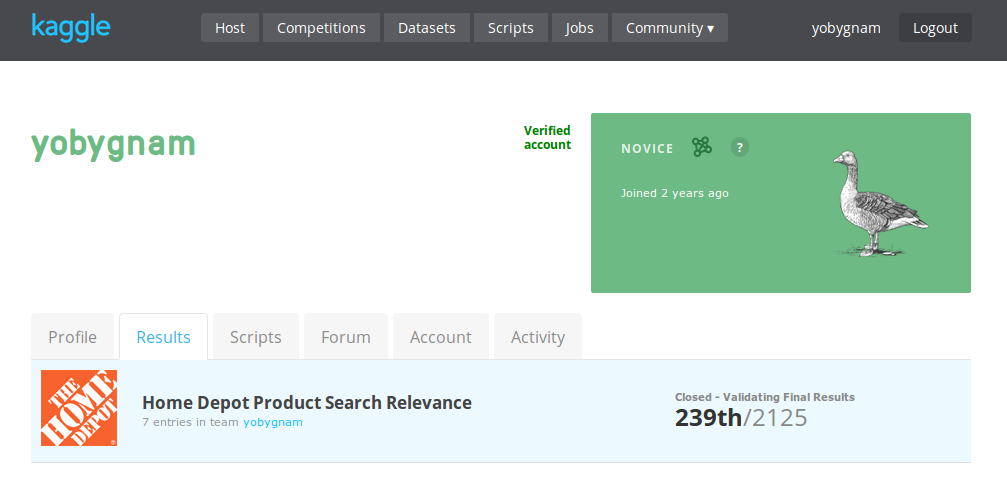
\includegraphics[scale=.43]{DataVisualization/kaggle_hd_aj_my_results.png} 
	\caption{Rank in Kaggle Home Depot Product Relevance Search Competition for my submission }
	\label{kag_my_rs}
\end{figure}

\FloatBarrier
\begin{figure}[!htbp]
	\centering
	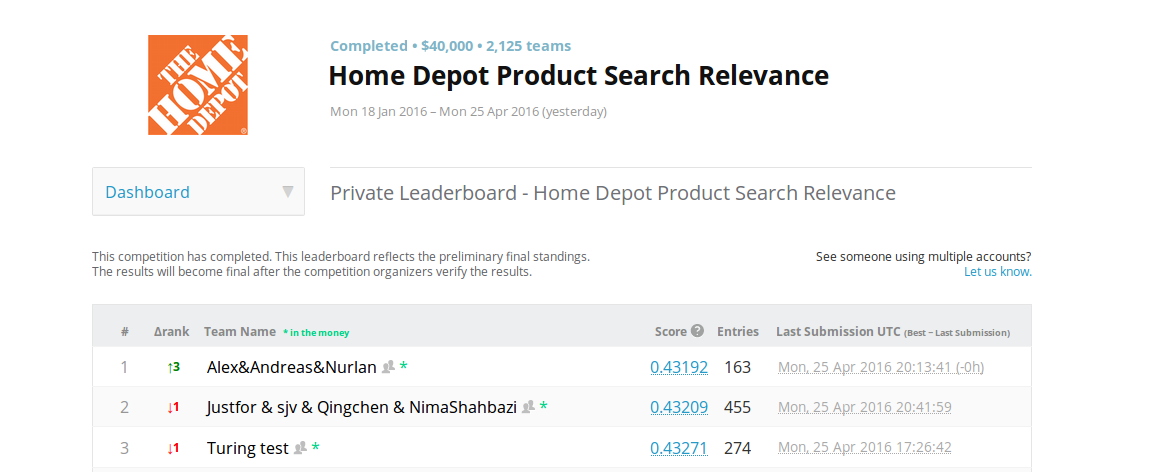
\includegraphics[scale=.43]{DataVisualization/kaggle_hd_all_results.png} 
	\caption{Top Rank results in Kaggle Home Depot Product Relevance Search Competition}
	\label{kag_top_rs}
\end{figure}

\subsection{Results for Project test set}
\FloatBarrier
\item
We created a hold out test set from the training data provide from Kaggle for this project. The RMSE error on that data set was 0.4672668171284915
\item
The optimum values of parameters chosen by  10 fold cross validation for Extreme Gradient Boosting Regressor are in table $\eqref{c_opt_params_bm}$
\FloatBarrier
\begin{table}[h]
	\centering
	\resizebox{\textwidth}{!}{
		\begin{tabular}{|c|c|c|c|c|}
			\hline
			&  Extreme Gradient Boosting Regressor & Gradient Boosting Regressor & Lasso & Random Forest Regressor \\
			\hline
			Optimum Parameters Chosen by 10-Fold Cross Validation & \begin{tabular}{@{}c@{}}estimators   600\\ learning rate       0.01\\gamma  0\\max\_depth 5\\subsample all\\ features all\end{tabular}  & \begin{tabular}{@{}c@{}}estimators 400\\ learning rate 0.05\\ max\_leaf\_nodes 5\\ features all \\ subsample all\end{tabular} & \begin{tabular}{@{}c@{}}alpha 0.001\end{tabular}&  \begin{tabular}{@{}c@{}}estimators 200\\max\_leaf\_nodes 4\\features all\\sample all\end{tabular}  \\
			\hline
		\end{tabular}
	}
	\caption[]{Optimum model Parameters chosen by 10-Fold Cross Validation }
	\label{c_opt_params_bm}
\end{table}

\FloatBarrier
\item
Table $\eqref{r_proj_error_models}$ tabulates the test error rate for predictions performed with the optimum parameters for each model on the hold out project test set. The Extreme Gradient Boosting has the best performance , followed by Gradient Boosting Regressor, Random Forest Regressor and finally Lasso.
\begin{table}[h]
\centering
\resizebox{\textwidth}{!}{
	\begin{tabular}{|c|c|c|c|c|c|c|c|}
		\hline
		& Extreme Gradient Boosting Regressor & Random Forest Regressor & Gradient Boosting Regressor & Lasso \\
		\hline
		 Project Test Error Rate & 0.4672668 & 0.472557 & 0.468457 & 0.477327  \\
		\hline
	\end{tabular}
	}
	\caption[]{Test Error Rate for the models on the Project hold out test set}
	\label{r_proj_error_models}
\end{table}
\end{itemize}

\FloatBarrier
\subsection{Top Features}
\begin{itemize}
\FloatBarrier
\item
Figure $\eqref{top_feat_rfr}$, $\eqref{top_feat_gbr}$ and $\eqref{top_feat_xgbr}$ list the top 20 features as seen by the Random Forest Regressor, Gradient Boosting Regressor and the Extreme Gradient Boosting Regressor respectively. The models seem to concur that the useful features are those engineered for word and segments in search string matching with those in the title. Both boosting models find the reduced dimensions of the tf-idf matrix for search string segments matching those in title take most of the top 20 places. So these plots suggest that search segment and title are mostly what relevance score is based on in this data set.
\FloatBarrier.
\begin{figure}[!htbp]
	\centering
	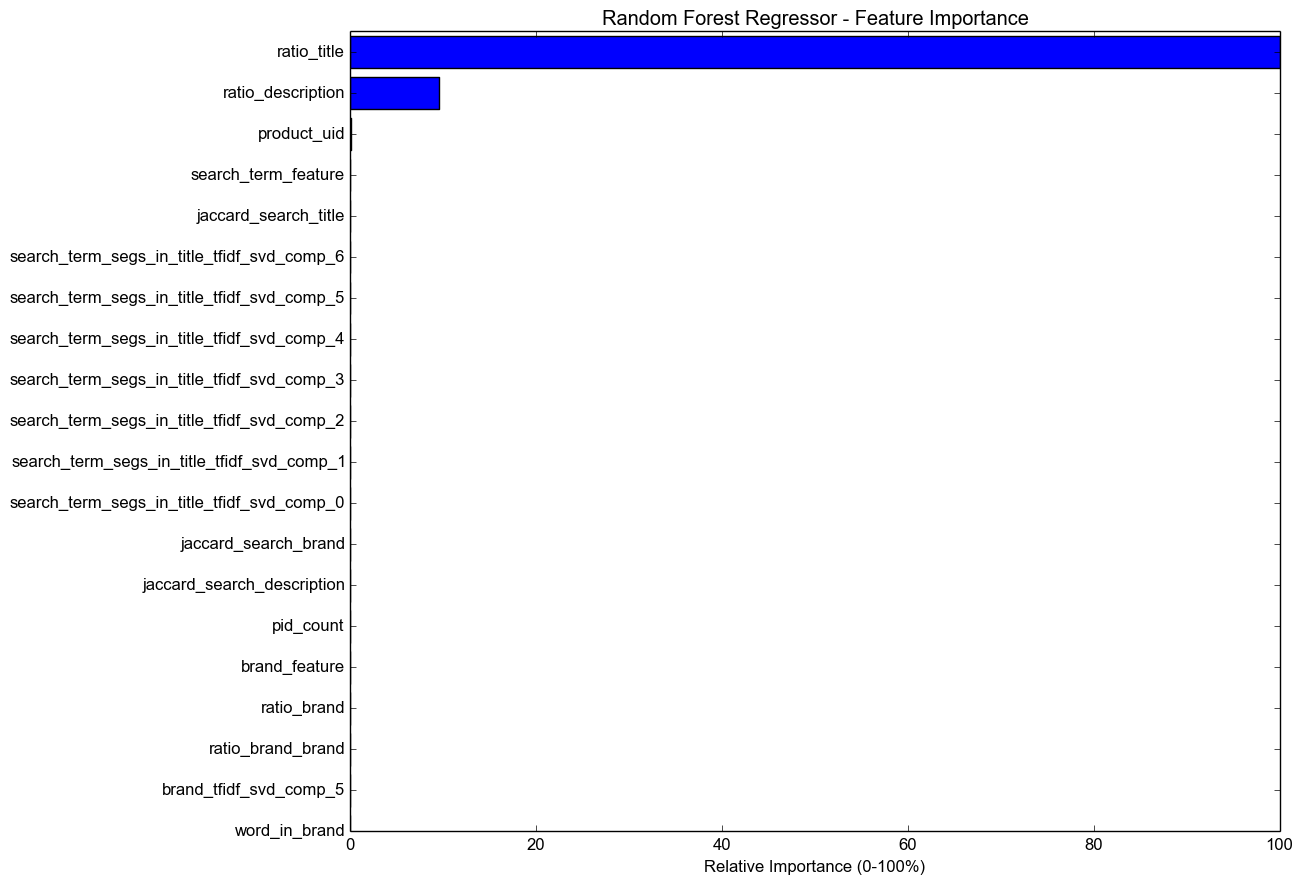
\includegraphics[scale=.43]{DataVisualization/rfr_fp.png} 
	\caption{Top features from the Random Forest Regressor}
	\label{top_feat_rfr}
\end{figure}
\begin{figure}[!htbp]
	\centering
	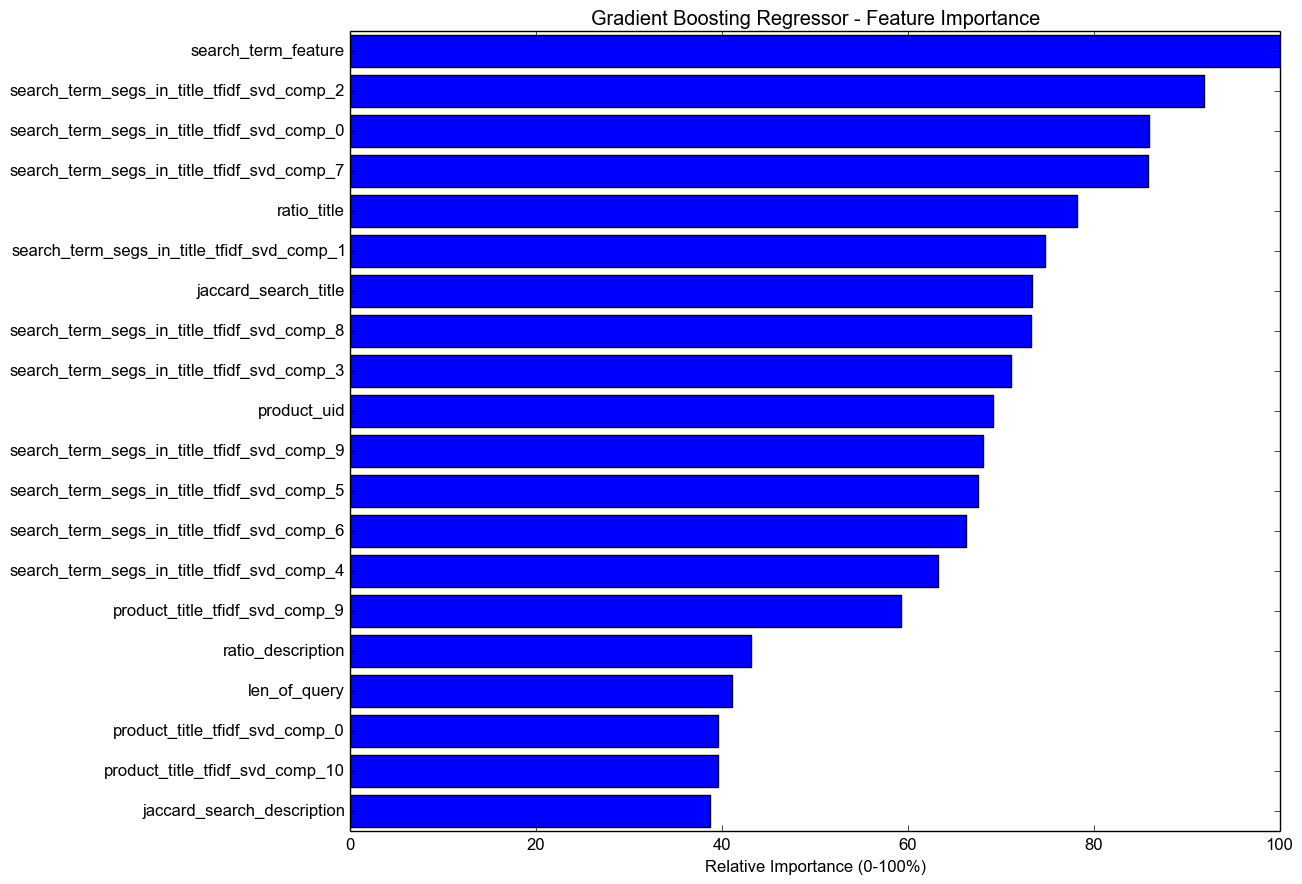
\includegraphics[scale=.43]{DataVisualization/gbr_fp.png} 
	\caption{Top 20 features from the Gradient Boosting Regressor}
	\label{top_feat_gbr}
\end{figure}
\begin{figure}[!htbp]
\centering
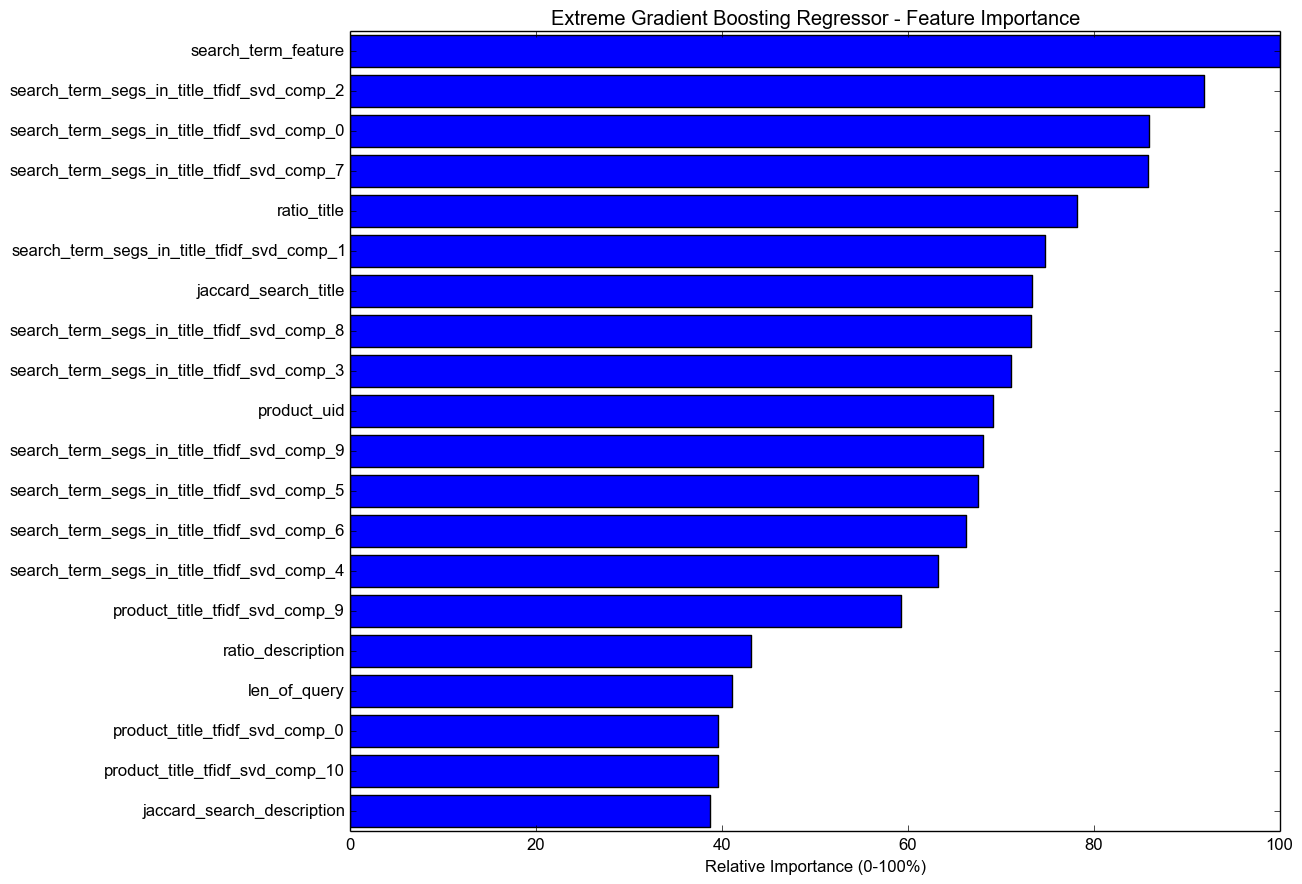
\includegraphics[scale=.43]{DataVisualization/xgbr_fp.png} 
\caption{Top 20 features from the Extreme Gradient Boosting Regressor}
\label{top_feat_xgbr}
\end{figure}

\end{itemize}


\FloatBarrier
\subsection{Cross Validation Plots - Extreme Gradient Boosting Regressor}
\begin{itemize}
\item
Figure $\eqref{top_cv_plot_1_xgbr}$ is a 3D plot of the CV results for Extreme Gradient Boosting Regressor. RMSE is plotted against n\_estimators/ and $\gamma$ for different learning rates. The tree\_depth is held constant at the prior chosen optimum value of 5. A low learning rate a large number of estimators seem to provide the optimum combination of parameters.
\begin{figure}[!htbp]
	\centering
	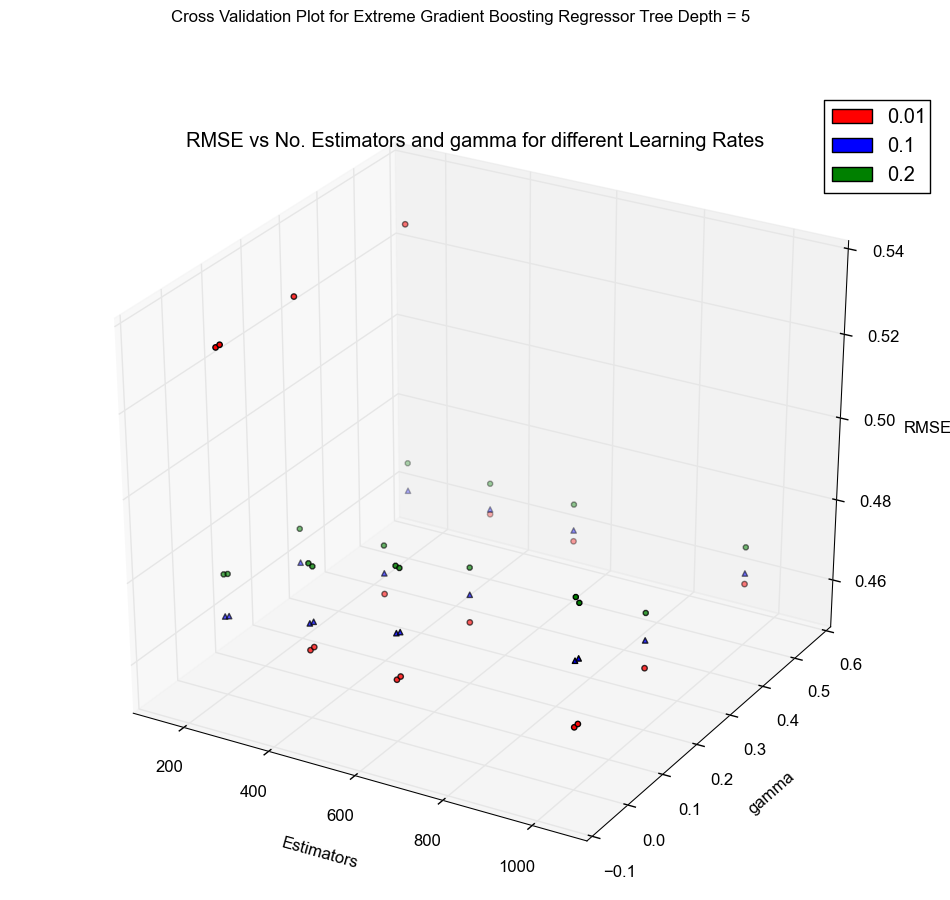
\includegraphics[scale=.43]{DataVisualization/3dplot_xgbr.png} 
	\caption{Cross Validation Results for n\_estimators,gamma,learning rate for Extreme Gradient Boosting Regressor}
	\label{top_cv_plot_1_xgbr}
\end{figure}


\FloatBarrier
\item
Figure $\eqref{n_est_gbr}$ and $\eqref{n_est_xgbr}$ is a plot the training and test RMSE as the number of estimators is increased for both the Gradient Boosting Regressor and the Extreme Gradient Boosting Regressor. The other parameters for the models are set to their optimum values as given in table $\eqref{c_opt_params_bm}$. Plots show that training error and test error rates form an elbow at around 200 estimators, further increase in the number of estimators shows very little reduction in test error rate. However for the  Gradient Boosting Regressor the training error rate does decline as the number of estimators is further increased, indicating that  Gradient Boosting Regressor since it does not have a penalty on the model complexity might have a tendency to overfit in comparison with the Extreme Gradient Boosting Regressor.
 n\_estimators/tree\_depth/learning rate
\begin{figure}[!htbp]
	\centering
	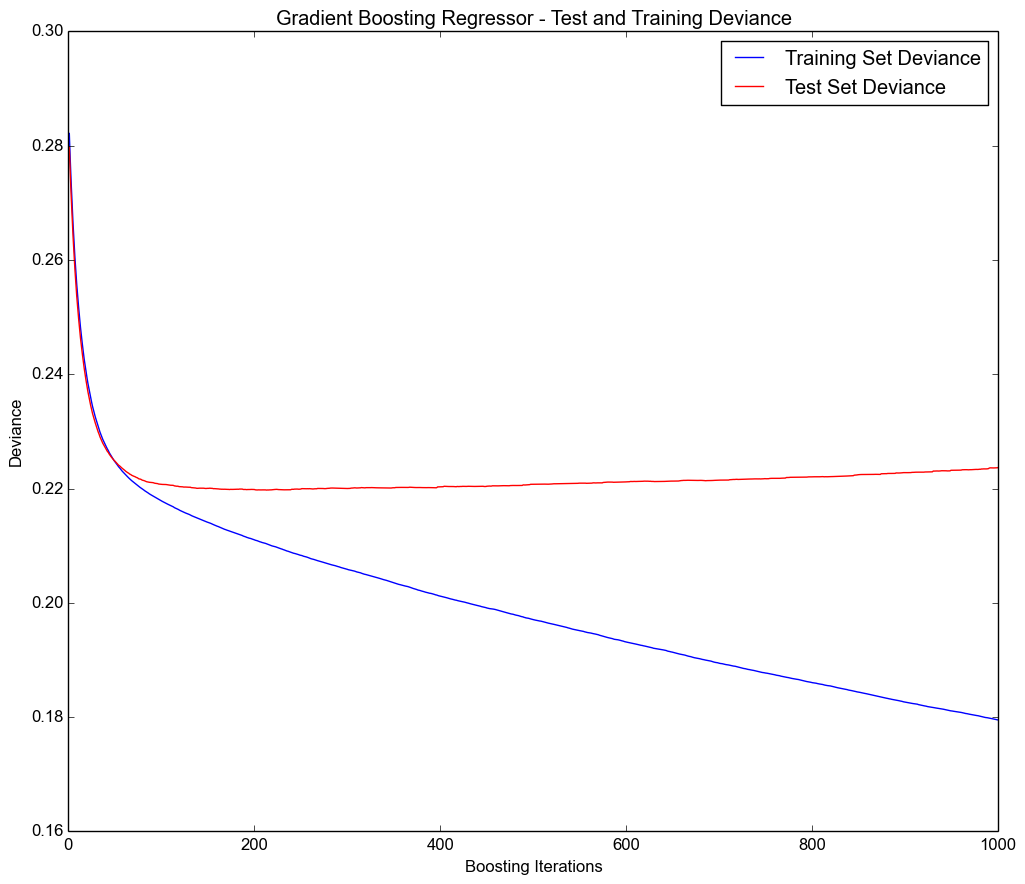
\includegraphics[scale=.43]{DataVisualization/gbr_ed_n.png} 
	\caption{Training and Test error rate Vs n\_estimators for Gradient Boosting Regressor}
	\label{n_est_gbr}
\end{figure}
\begin{figure}[!htbp]
	\centering
	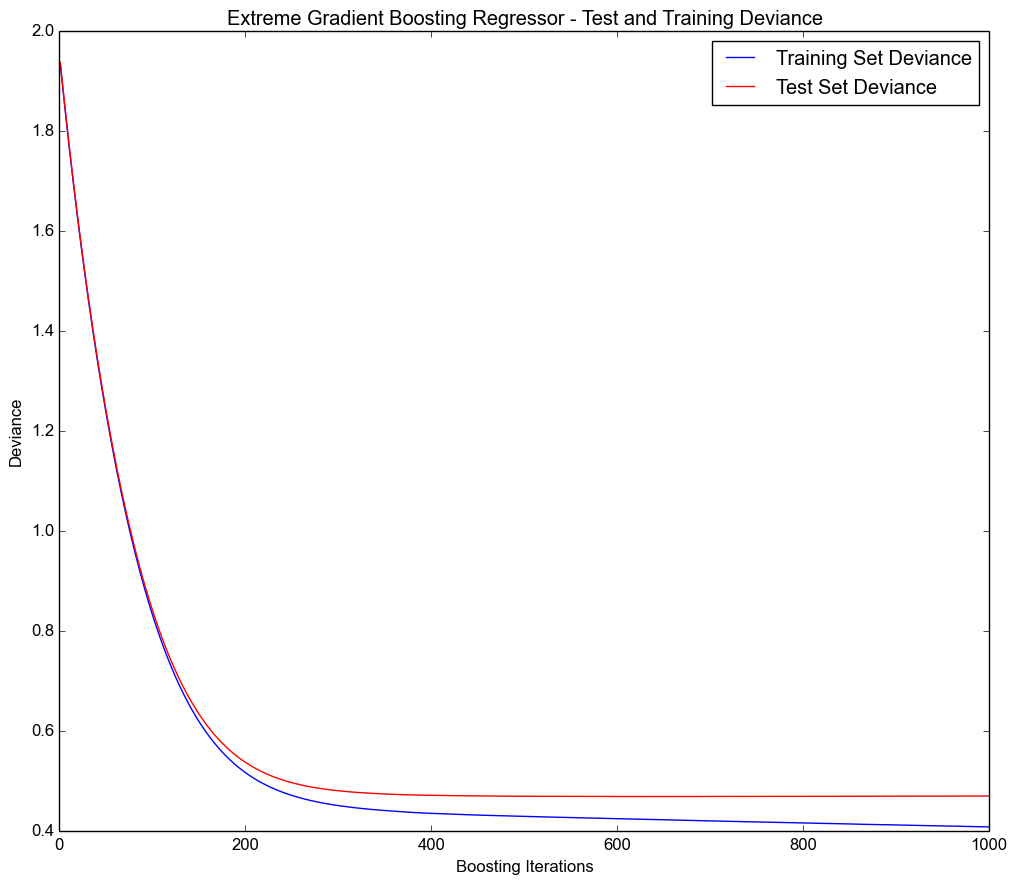
\includegraphics[scale=.43]{DataVisualization/xgbr_ed_n.png} 
	\caption{Training and Test error rate Vs n\_estimators for Extreme Gradient Boosting Regressor}
	\label{n_est_xgbr}
\end{figure}

\FloatBarrier
\subsection{Choosing the best model - Bootstrapping Results}
\FloatBarrier
\item
As discussed earlier the best model for submission will be chosen based on bootstrapping results. We performed a 30 iteration bootstrapping with a random $40\%$ of data chosen with replacement as the test set and the remaining as the training set. Figure $\eqref{bs_models}$ is the box plot of the bootstrapping results. The Extreme Gradient Boosting Regressor performed the best on the test set,
\begin{figure}[!htbp]
\centering
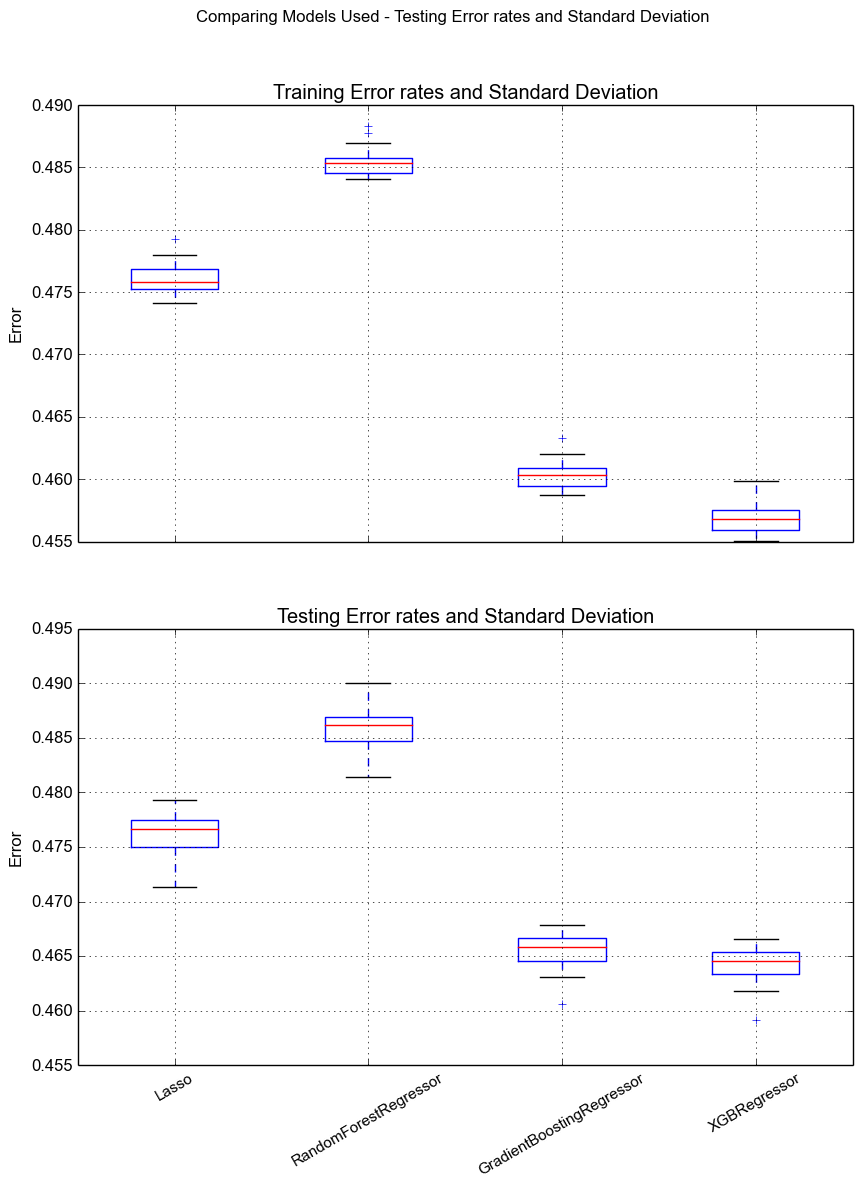
\includegraphics[scale=.65]{DataVisualization/models.png} 
\caption{Boxplot of B=300 Bootstraping results}
\label{bs_models}
\end{figure}


\FloatBarrier
\subsubsection{T-test and Wilcox Test for choosing the best model}
	\item
	We performed a statistical T-test as well a a Wilcox test to confirm that the Extreme Gradient Boosting Regressor results was the best model based on the bootstrapping test set results.
		\item
		Table $\eqref{r_tab_bs_results}$ tabulates the T-test and Wilcox 2 sample paired test results between Extreme Gradient Boost Regressor and every other method. The $P-Values$ are very low for significance level of $\alpha = 5\%$. This leads us to to reject the NULL hypothesis at the significance level of $\alpha = 5\%$ and strongly conclude that Extreme Gradient Boost Regressor is the best model trained for this dataset.
		\FloatBarrier
		\begin{table}[h]
			\centering
			\resizebox{\textwidth}{!}{
				\begin{tabular}{|c|c|c|c|}
					\hline
					& RandomForestRegressor & GradientBoostingRegressor & Lasso \\
					\hline
					T-Test & 1.0701507e-47 & 0.0074 & 3.12418e-34 \\
					\hline
					Wilcox Test & 1.7343976e-06 & 1.734397e-06 & 1.734397e-06 \\
					\hline
				\end{tabular}
			}
			\caption[]{T-test and Wilcox Test comparing Error rate of Extreme Gradient Boost Regressor with other Regression models used }
			\label{r_tab_bs_results}
		\end{table}
\end{itemize}



\FloatBarrier
\section{Conclusions}
\label{Conclusions}

\FloatBarrier
\begin{itemize}
\item
Understanding the domain, exploring and analyzing the data are the most important steps for engineering good features to train a model on. In this competition there where no ready features provided, the input was text data and engineering features was left to ones ingenuity and imagination.
\item
A good and well instrumented feature matrix, that is a faithful representation of the data is most crucial for performing any learning on the data
\item
While various training models have different assumptions, they will still do a reasonably decent job on a  very well engineered feature vector, but the reverse is not true. Even the best and most appropriate model will do a poor job of learning on poor feature vector that does not represent the data very well
\item
Given a well engineered feature vector and an appropriate model, one still needs to perform a exhaustive search for the most optimum model parameters. This process is time and resource intensive and is best done in parallel on a distributed system. A single CPU PC is not a great tool for this purpose and will not permit an exhaustive search with cross validation on even a medium sized data set
\item
As expected training error rate is lower than test error rate for all models. 
\item
Beyond a certain threshold of ensembles the models will over fit the training data unless penalized.
\item
For this competition Cross Validation and Bootstrapping are the primary tools used to train and evaluate the models and seem to be the default methods to do so.
\item
Ensemble models with boosting which have a penalty for model complexity in their objective function are a fairly robust learning model as they have the mechanism to best balance bias variance tradeoff right into the objective function
\item
Boosting methods since they add learners in series are slower than pure ensemble methods which can take advantage of parallel processing to train and independent learners. However boosting methods are better on bias while non boosted ensembles trade bias for variance.
\end{itemize}

\FloatBarrier


\subsection{Lessons from the Project}
\begin{itemize}
	\item
	From the point of view of the competition the top 10 submissions as well as most of the top 200 ranks where taken by teams of more than 1. Competing as a team in competitions like this gives an advantage for trying new ideas and working on them in parallel
	\item
	One needs to go deeper with engineering features and go wider in searching for optimum parameters when fitting models on this trained data. 
	\item
	An exhaustive search for optimum parameters on a grid of parameter value ranges using a ten fold cross validation is a slow and time consuming process. One needs to have an efficient strategy on perform this computation as it is crucial for fine training the model for a competition like this. Parallel and distributed computing on a cloud environment is the best way to perform this computation both for speed and efficiency and precision of the project.
\end{itemize}

\FloatBarrier
\section{Appendix}
\label{Appendix}
\begin{enumerate}
\item
The python source code used for performing the data analysis and for engineering the feature vectors for the this project is in file $ajdsouza31-hd\_rf\_featurize.py$, which is submitted on $T-Square$ along with this report.
\item
The python source code for training the models, choosing the best model and for generating the test results for submission to the Kaggle competition is in file $ajdsouza31-hd\_rf.py$, which is submitted on $T-Square$ along with this report.
\item
The following is the URL for the Kaggle Home Depot Product Search Relevance competition. The test and training data sets are available at this link
\url{https://www.kaggle.com/c/home-depot-product-search-relevance}
\end{enumerate}



%\addcontentsline{toc}{section}{References}
\bibliographystyle{plain}
% Generate the bibliography.
\begin{thebibliography}{9}

\bibitem{hastie_2009}
  Trevor Hastie, Robert Tibshirani, Jerome Friedman,
  \emph{\LaTeX: Elements of Statistical Learning},
  Elements of Statistical Learning Ed. 2,
  2009.

\bibitem[Friedman(2001)]{fried1}
	J.H. Friedman.
	\newblock Greedy function approximation: a gradient boosting machine.
	\newblock \emph{The Annals of Statistics}, 29:\penalty0 1189--1232, 2001.

\bibitem[Friedman et~al.(2000)Friedman, Hastie, and Tibshirani]{fht}
	J.H. Friedman, T.~Hastie, and R.~Tibshirani.
	\newblock Additive logistic regression: a statistical view of boosting (with discussion).
	\newblock \emph{The Annals of Statistics}, 28:\penalty0 337--407, 2000.

\bibitem[Pedregosa et~al., 2011]{sklearn}
 Pedregosa, F., Varoquaux, G., Gramfort, A., Michel, V., Thirion, B., Grisel,
    O., Blondel, M., Prettenhofer, P., Weiss, R., Dubourg, V., Vanderplas, J.,
    Passos, A., Cournapeau, D., Brucher, M., Perrot, M., and Duchesnay, E.
    (2011).
 \newblock Scikit-learn: Machine learning in {P}ython.
 \newblock {\em Journal of Machine Learning Research}, 12:2825--2830 

\bibitem[Zhang and Yu(2005)]{zhyu}
	T.~Zhang and B.~Yu.
	\newblock Boosting with early stopping: convergence and consistency.
	\newblock \emph{The Annals of Statistics}, 33:\penalty0 1538--1579, 2005.

\end{thebibliography}

\end{document}